\documentclass[]{article}
\usepackage{lmodern}
\usepackage{amssymb,amsmath}
\usepackage{ifxetex,ifluatex}
\usepackage{fixltx2e} % provides \textsubscript
\ifnum 0\ifxetex 1\fi\ifluatex 1\fi=0 % if pdftex
  \usepackage[T1]{fontenc}
  \usepackage[utf8]{inputenc}
\else % if luatex or xelatex
  \ifxetex
    \usepackage{mathspec}
  \else
    \usepackage{fontspec}
  \fi
  \defaultfontfeatures{Ligatures=TeX,Scale=MatchLowercase}
\fi
% use upquote if available, for straight quotes in verbatim environments
\IfFileExists{upquote.sty}{\usepackage{upquote}}{}
% use microtype if available
\IfFileExists{microtype.sty}{%
\usepackage{microtype}
\UseMicrotypeSet[protrusion]{basicmath} % disable protrusion for tt fonts
}{}
\usepackage[margin=1in]{geometry}
\usepackage{hyperref}
\hypersetup{unicode=true,
            pdftitle={Critical Plot Analysis},
            pdfauthor={Joao Pedro Oliveira},
            pdfborder={0 0 0},
            breaklinks=true}
\urlstyle{same}  % don't use monospace font for urls
\usepackage{graphicx,grffile}
\makeatletter
\def\maxwidth{\ifdim\Gin@nat@width>\linewidth\linewidth\else\Gin@nat@width\fi}
\def\maxheight{\ifdim\Gin@nat@height>\textheight\textheight\else\Gin@nat@height\fi}
\makeatother
% Scale images if necessary, so that they will not overflow the page
% margins by default, and it is still possible to overwrite the defaults
% using explicit options in \includegraphics[width, height, ...]{}
\setkeys{Gin}{width=\maxwidth,height=\maxheight,keepaspectratio}
\IfFileExists{parskip.sty}{%
\usepackage{parskip}
}{% else
\setlength{\parindent}{0pt}
\setlength{\parskip}{6pt plus 2pt minus 1pt}
}
\setlength{\emergencystretch}{3em}  % prevent overfull lines
\providecommand{\tightlist}{%
  \setlength{\itemsep}{0pt}\setlength{\parskip}{0pt}}
\setcounter{secnumdepth}{0}
% Redefines (sub)paragraphs to behave more like sections
\ifx\paragraph\undefined\else
\let\oldparagraph\paragraph
\renewcommand{\paragraph}[1]{\oldparagraph{#1}\mbox{}}
\fi
\ifx\subparagraph\undefined\else
\let\oldsubparagraph\subparagraph
\renewcommand{\subparagraph}[1]{\oldsubparagraph{#1}\mbox{}}
\fi

%%% Use protect on footnotes to avoid problems with footnotes in titles
\let\rmarkdownfootnote\footnote%
\def\footnote{\protect\rmarkdownfootnote}

%%% Change title format to be more compact
\usepackage{titling}

% Create subtitle command for use in maketitle
\newcommand{\subtitle}[1]{
  \posttitle{
    \begin{center}\large#1\end{center}
    }
}

\setlength{\droptitle}{-2em}

  \title{Critical Plot Analysis}
    \pretitle{\vspace{\droptitle}\centering\huge}
  \posttitle{\par}
    \author{Joao Pedro Oliveira}
    \preauthor{\centering\large\emph}
  \postauthor{\par}
      \predate{\centering\large\emph}
  \postdate{\par}
    \date{11/1/2018}


\begin{document}
\maketitle

\subsection{This is my critical analysis of a plot I found on the
web.}\label{this-is-my-critical-analysis-of-a-plot-i-found-on-the-web.}

This plot was originally posted by Bloomberg, which is a news outlet I
read quite regularly. I chose Bloomberg because I find their plots to be
quite creative, informative and very different from the other news
websites.

\begin{figure}
\centering
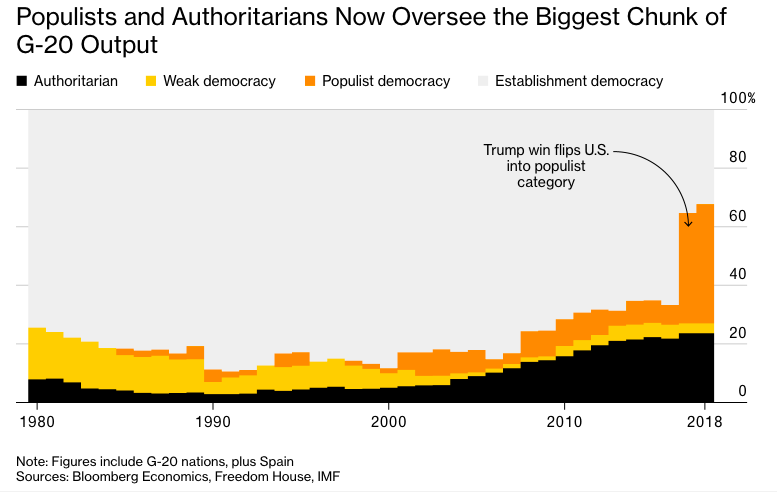
\includegraphics{plot.png}
\caption{}
\end{figure}

\subsubsection{\texorpdfstring{So, this is the plot. Some problems
emerge quickly in the interpretation of the plot though. Since the plot
has no labels for the X and Y axis, one must assume that based on the
title. I assumed that the Y axis is the percentage of the total G20
Economic Output and the X axis is the year. But the graph has another
information plotted in it, and that is the ``Political System'' that
rules the government of the
nations.}{So, this is the plot. Some problems emerge quickly in the interpretation of the plot though. Since the plot has no labels for the X and Y axis, one must assume that based on the title. I assumed that the Y axis is the percentage of the total G20 Economic Output and the X axis is the year. But the graph has another information plotted in it, and that is the Political System that rules the government of the nations.}}\label{so-this-is-the-plot.-some-problems-emerge-quickly-in-the-interpretation-of-the-plot-though.-since-the-plot-has-no-labels-for-the-x-and-y-axis-one-must-assume-that-based-on-the-title.-i-assumed-that-the-y-axis-is-the-percentage-of-the-total-g20-economic-output-and-the-x-axis-is-the-year.-but-the-graph-has-another-information-plotted-in-it-and-that-is-the-political-system-that-rules-the-government-of-the-nations.}

\paragraph{\texorpdfstring{What the plot is trying to tell us is quite
clear: Autoritarians and populists now oversee most of the G20 global
output. But another question arises from that, which is: ``how do you
define the type and status of a political system?'', or ``who defines
the type of a political system?''. How do you come to the conclusion
that a nation has a ``weak democracy''? You can have the opinion that
the U.S Government is not run by a Populist, or say that Venezuela isn't
an autoritharian
government.}{What the plot is trying to tell us is quite clear: Autoritarians and populists now oversee most of the G20 global output. But another question arises from that, which is: how do you define the type and status of a political system?, or who defines the type of a political system?. How do you come to the conclusion that a nation has a weak democracy? You can have the opinion that the U.S Government is not run by a Populist, or say that Venezuela isn't an autoritharian government.}}\label{what-the-plot-is-trying-to-tell-us-is-quite-clear-autoritarians-and-populists-now-oversee-most-of-the-g20-global-output.-but-another-question-arises-from-that-which-is-how-do-you-define-the-type-and-status-of-a-political-system-or-who-defines-the-type-of-a-political-system.-how-do-you-come-to-the-conclusion-that-a-nation-has-a-weak-democracy-you-can-have-the-opinion-that-the-u.s-government-is-not-run-by-a-populist-or-say-that-venezuela-isnt-an-autoritharian-government.}

\subsubsection{For this plot to be useful, in my opinion, the methods
that you used to gather and classify the data must be really
clear.}\label{for-this-plot-to-be-useful-in-my-opinion-the-methods-that-you-used-to-gather-and-classify-the-data-must-be-really-clear.}

\subsubsection{Other than that, I think the design of the plot is really
good, and it really carries the message that the newspaper is trying to
convey. Some color choices might have been on pourpose, like the white
color for the democratic governments since those were not the focus of
the message, and that might be a point for discussion, but that's just
fine for
me.}\label{other-than-that-i-think-the-design-of-the-plot-is-really-good-and-it-really-carries-the-message-that-the-newspaper-is-trying-to-convey.-some-color-choices-might-have-been-on-pourpose-like-the-white-color-for-the-democratic-governments-since-those-were-not-the-focus-of-the-message-and-that-might-be-a-point-for-discussion-but-thats-just-fine-for-me.}


\end{document}
